\chapter{django概述}

\section{概述}
\href{https://docs.djangoproject.com/en/3.0/}{3.0的官方文档}

\section{MVC模型}
MVC 模式（Model–view–controller）是软件工程中的一种软件架构模式，把软件系统分为三个基本部分：模型（Model）、视图（View）和控制器（Controller）。

MVC 以一种插件式的、松耦合的方式连接在一起。

Django 本身基于 MVC 模型，即 Model（模型）+ View（视图）+ Controller（控制器）设计模式，
MVC 模式使后续对程序的修改和扩展简化。

\begin{enumerate}[label=\arabic*)]
  \item 模型（Model）： 负责应用程序的数据和业务逻辑。通过将数据和逻辑从用户界面分离出来，使得模型可以独立于用户界面进行测试和修改。
  \item 视图（View）： 负责显示用户界面，但通常没有直接访问应用程序的数据。这使得可以更容易地更改应用程序的外观而不影响数据处理。
  \item 控制器（Controller）： 处理用户输入、更新模型和调整视图。通过将用户输入和应用程序逻辑分离，可以更容易地更改用户界面的交互方式而不影响数据和业务逻辑。
\end{enumerate}

\begin{figure}[htpb]
  \centering
  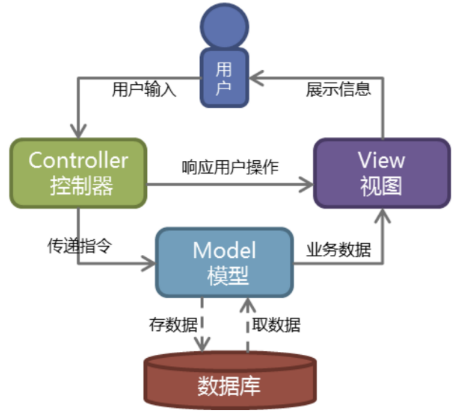
\includegraphics[width=0.4\textwidth]{part/互联/django/pic/概述/MVC模型示意图.png}
  \caption{MVC模型示意图}
  \label{fig:MVC模型示意图}
\end{figure}

\subsection{MTV模型}
Django 的 MTV 模式本质上和 MVC 是一样的，也是为了各组件间保持松耦合关系，只是定义上有些许不同，Django 的 MTV 分别是指：
\begin{enumerate}[label=\arabic*)]
  \item M 表示模型（Model）：编写程序应有的功能，负责业务对象与数据库的映射(ORM)。
  \item T 表示模板 (Template)：负责如何把页面(html)展示给用户。
  \item V 表示视图（View）：负责业务逻辑，并在适当时候调用 Model和 Template。
\end{enumerate}

除了以上三层之外，还需要一个 URL 分发器，它的作用是将一个个 URL 的页面请求分发给不同的 View 处理，View 再调用相应的 Model 和 Template。


\subsection{Django的工作流程}
\begin{figure}[htpb]
  \centering
  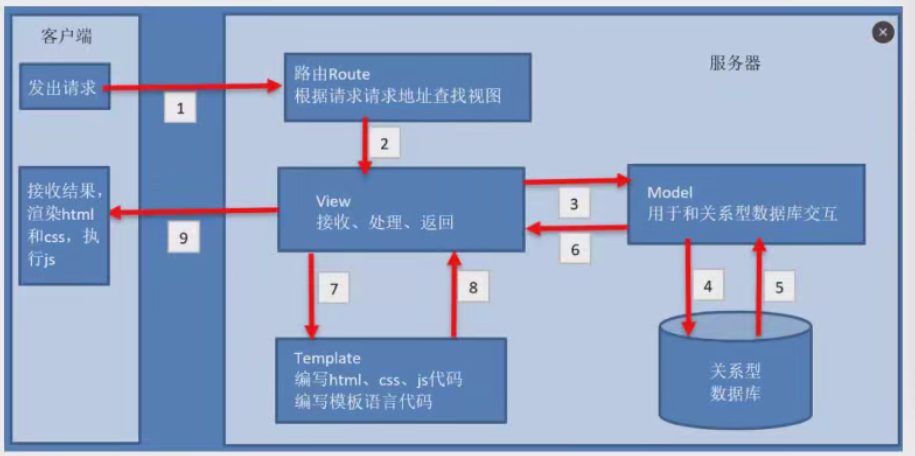
\includegraphics[width=0.4\textwidth]{part/互联/django/pic/概述/Django流程.png}
  \caption{Django流程}
  \label{fig:Django流程}
\end{figure}

\begin{enumerate}[label=\arabic*)]
  \item 浏览器通过域名发送一个 HTTP 请求到 Django 服务器。
  \item 路由(URLconf)接收到请求，网站的功能模块被映射到一个 URL(路由)。
  \item django根据请求的URL调用相应的视图函数(views)。
  \item 视图函数处理请求，可能会与数据库交互，然后返回一个 HTTP 响应。

  \begin{enumerate}[itemindent=1em,label=\arabic*)]
    \item 数据模型(Model)：与数据库交互，处理数据。
    \item 当数据模型获取到数据后，视图函数将数据传递给模板(template,存储前端的html文件)。
    \item 模板将数据渲染到前端页面。
  \end{enumerate}
  
  \item Django 将响应发送回浏览器，浏览器将其呈现给用户。
\end{enumerate}


\section{Django的安装}
\subsection{conda安装}
\begin{lstlisting}[style=demostyle,numbers=none]
$> conda create --name mydjango python=3.10
$> conda activate mydjango
$> conda install django==3.0.3
$ python3 -m django --version
3.0.3
\end{lstlisting}

\subsection{pip安装}
\begin{lstlisting}[style=demostyle,numbers=none]
$> sudo pip3 install Django -i https://pypi.tuna.tsinghua.edu.cn/simple
$> sudo pip3 install Django==3.0.6 -i https://pypi.tuna.tsinghua.edu.cn/simple
\end{lstlisting}



\section{主项目}
\subsection{创建项目}
\begin{lstlisting}[style=demostyle,numbers=none]
$> django-admin startproject recruitment_demo
$> tree
|-- manage.py # 命令行工具, 用于管理项目
`-- recruitment_demo # 项目的容器
    |-- __init__.py # 一个空文件，告诉 Python 该目录是一个 Python 包
    |-- __pycache__ # 编译后的文件
    │   |-- __init__.cpython-310.pyc
    │   |-- settings.cpython-310.pyc
    │   |-- urls.cpython-310.pyc
    │   `-- wsgi.cpython-310.pyc
    |-- asgi.py # 一个 ASGI 兼容的 Web 服务器入口点
    |-- settings.py # 项目的配置文件
    |-- urls.py # 项目的 URL 声明, 一份由 Django 驱动的网站"目录"
    `-- wsgi.py # 一个 WSGI 兼容的 Web 服务器的入口点
\end{lstlisting}
\subsection{查询帮助}
\begin{lstlisting}[style=demostyle,numbers=none]
$> python manage.py help
Type 'manage.py help <subcommand>' for help on a specific subcommand.

Available subcommands:

[auth]
    changepassword
    createsuperuser

[contenttypes]
    remove_stale_contenttypes

[django]
    check
    compilemessages
    createcachetable
    dbshell
    diffsettings
    dumpdata
    flush
    inspectdb
    loaddata
    makemessages
    makemigrations
    migrate
    sendtestemail
    shell
    showmigrations
    sqlflush
    sqlmigrate
    sqlsequencereset
    squashmigrations
    startapp
    startproject
    test
    testserver

[sessions]
    clearsessions

[staticfiles]
    collectstatic
    findstatic
    runserver
\end{lstlisting}

\begin{enumerate}[label=\arabic*)]
  \item auth：用户认证系统,与 Django 的认证系统（用户、权限、组等）相关
  \begin{enumerate}[itemindent=1em,label=\arabic*)]
    \item \codeinline{changepassword}：修改用户密码。
    \item \codeinline{createsuperuser}：创建超级用户。
  \end{enumerate}

  \item contenttypes：内容类型框架相关，内容类型框架允许你以统一的方式处理不同类型的模型。
  \begin{enumerate}[itemindent=1em,label=\arabic*)]
    \item \codeinline{remove\_stale\_contenttypes}：删除无用的内容类型。
  \end{enumerate}
  
  \item django：Django 管理命令,涉及数据库迁移、开发环境管理、数据导入导出等。
  \begin{enumerate}[itemindent=1em,label=\arabic*)]
    \item \codeinline{check}：检查 Django 项目中是否存在任何错误或潜在问题。适用于快速检测项目状态。
    \item \codeinline{compilemessages}：编译 Django 项目中的翻译文件（.po 文件转 .mo 文件）。用于多语言支持。
    \item \codeinline{createcachetable}：创建数据库表以便使用缓存系统。用于缓存的数据库存储。
    \item \codeinline{dbshell}：打开一个数据库 shell（命令行界面），可以直接操作项目的数据库。
    \item \codeinline{diffsettings}：显示当前项目配置与默认配置的差异，帮助你查看哪些设置被修改过。
    \item \codeinline{dumpdata}：将数据库中的数据导出为 JSON 格式，通常用于备份或者数据迁移。
    \item \codeinline{flush}：重置数据库，将所有的数据清除并恢复到初始状态。会清空所有表，通常用于开发时清理数据。
    \item \codeinline{inspectdb}：根据现有的数据库表生成对应的 Django 模型代码（即反向生成模型）。
    \item \codeinline{loaddata}：加载之前导出的数据文件（通常是 JSON 格式）到数据库中。
    \item \codeinline{makemessages}：扫描代码，查找需要翻译的字符串，并生成相应的翻译文件（.po）。
    \item \codeinline{makemigrations}：生成数据库迁移文件，记录模型的更改。迁移是 Django 对数据库结构变化的管理。
    \item \codeinline{migrate}：应用迁移文件，更新数据库结构，使其与当前的模型状态一致。
    \item \codeinline{sendtestemail}：发送一个测试电子邮件，用于测试邮件设置是否正常。
    \item \codeinline{shel}l：启动 Django 的交互式 Python shell，允许你直接在命令行中操作 Django 项目，例如查询数据库、操作模型等。
    \item \codeinline{showmigrations}：显示当前数据库迁移的状态，哪些迁移已应用，哪些没有应用。
    \item \codeinline{sqlflush}：生成并显示清空数据库表（flush）所需要的 SQL 语句。
    \item \codeinline{sqlmigrate}：查看某个迁移文件对应的 SQL 语句。
    \item \codeinline{sqlsequencereset}：查看重置数据库表的序列（主要是用于自增字段）所需要的 SQL 语句。
    \item \codeinline{squashmigrations}：将多个迁移合并为一个迁移文件，帮助减少迁移文件的数量。
    \item \codeinline{startapp}：创建一个新的 Django 应用，并生成默认的目录结构。
    \item \codeinline{startproject}：创建一个新的 Django 项目，初始化基本的项目结构。
    \item \codeinline{test}：运行 Django 测试框架中的测试，通常用于验证你的代码是否正常工作。
    \item \codeinline{testserver}：启动一个测试服务器，用于测试环境中的调试和运行。
  \end{enumerate}
  

  
\end{enumerate}



\subsection{启动项目}
\begin{lstlisting}[style=demostyle,numbers=none]
$> python manage.py runserver ip地址:端口

# 本地访问
$> python manage.py runserver 0.0.0.0:8000
\end{lstlisting}

然后访问\codeinline{http://localhost:8000/}，可以看到如图\ref{fig:Django启动成功}所示的页面。
\begin{figure}[htpb]
  \centering
  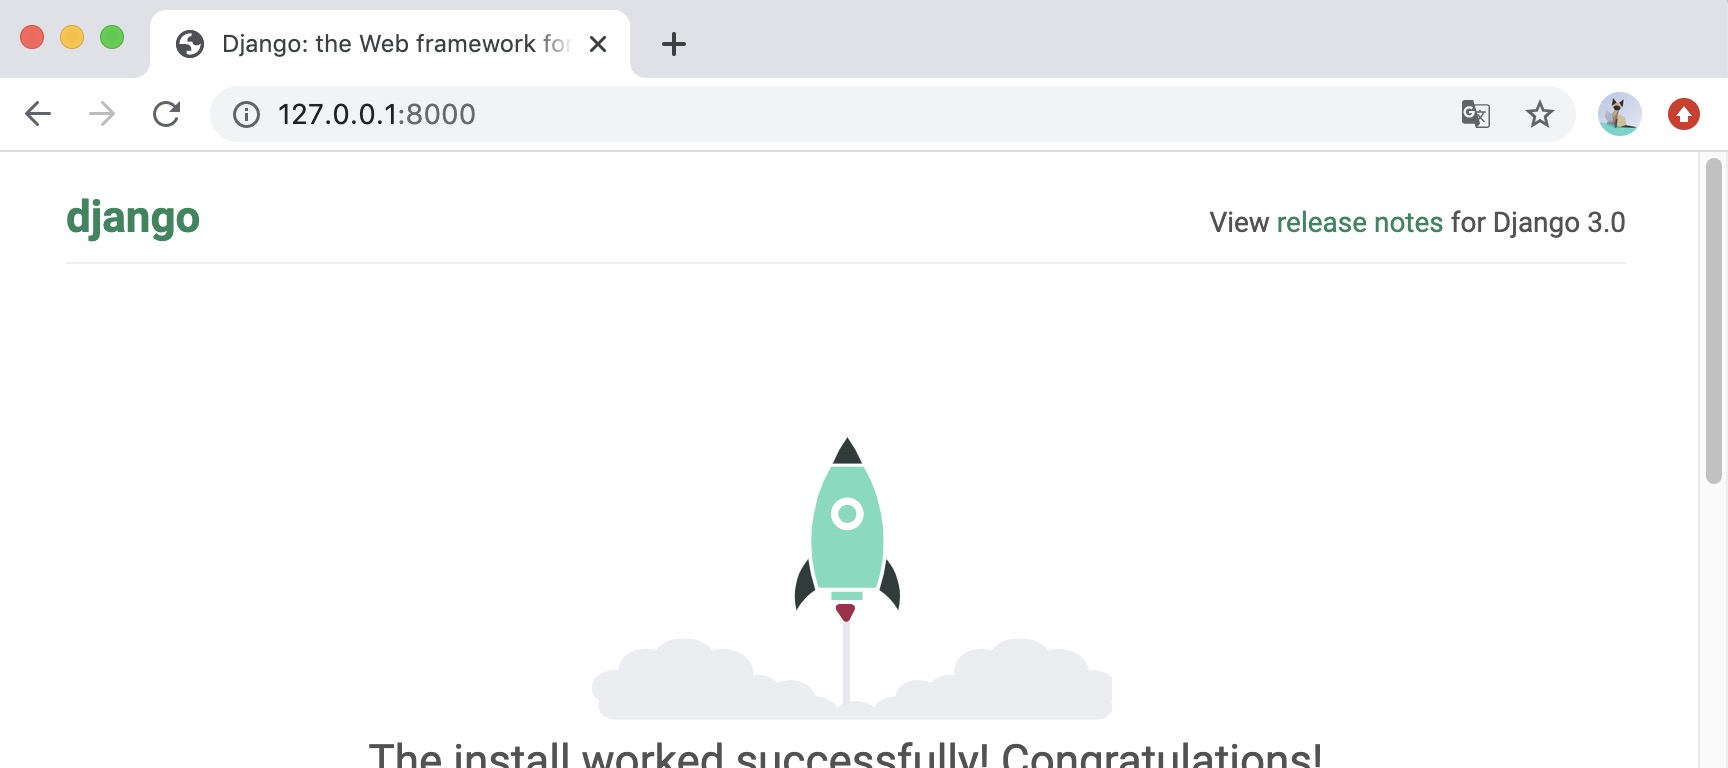
\includegraphics[width=0.4\textwidth]{part/互联/django/pic/概述/Django启动成功.png}
  \caption{Django启动成功}
  \label{fig:Django启动成功}
\end{figure}



\section{创建子应用}
\subsubsection{子应用的作用}
\begin{example}
  \exProblem
  Django的主项目相当一家公司，公司下面有很多部门：开发部、运营部、财务部等等。
  
  \begin{enumerate}[label=\arabic*)]
    \item 公司->主项目
    \item 部门->子应用
  \end{enumerate}
  
  每个子应用之间相互独立，可以单独运行，也可以被其他项目引用。
\end{example}

\subsection{创建子应用}
\begin{lstlisting}[style=demostyle,numbers=none]
$> python manage.py startapp 子应用名称
\end{lstlisting}

\begin{lstlisting}[style=demostyle,numbers=none]
$> python manage.py startapp jobs
$> tree
|-- manage.py
|-- recruitment_demo # 主项目的容器
│   |-- __init__.py
...
`-- jobs  # 子应用的文件夹
    |-- __init__.py
    |-- admin.py  # 管理后台
    |-- apps.py   # 子应用的配置文件
    |-- migrations # 数据库迁移文件
    │   `-- __init__.py
    |-- models.py
    |-- tests.py   # 单元测试
    `-- views.py   # 视图函数
\end{lstlisting}

\subsection{注册子应用}
在主项目的\codeinline{settings.py}文件中注册子应用。
\begin{lstlisting}[style=demostyle,numbers=none]
$> ls 
jobs  recruitment_demo  
$> cat recruitment_demo/settings.py # recruitment_demo是主项目的文件夹名称  
INSTALLED_APPS = [
    'django.contrib.admin',
    'django.contrib.auth',
    'django.contrib.contenttypes',
    'django.contrib.sessions',
    'django.contrib.messages',
    'django.contrib.staticfiles',
    'jobs',  # 注册子应用, jobs是子应用的文件夹名称
    # 或者
    'job.apps.JobConfig',  # 注册子应用, job是子应用的文件夹名称
]
\end{lstlisting}

在注册子应用有两种写法
\begin{enumerate}[label=\arabic*)]
  \item \codeinline{'子模块名'}

  这种写法会自动加载子应用的配置文件\codeinline{apps.py}，并执行其中的代码。

  \item \codeinline{'子模块名.apps.子模块名Config'}

  这个\codeinline{子模块名Config}是\codeinline{apps.py}中个一个类，一般约定的写法。

  该方法显式指定应用的配置入口，Django 会加载该配置，而不是使用默认配置。
  可以在\codeinline{子模块名Config}中定义一些特定的行为
\begin{lstlisting}[style=demostyle,numbers=none]
class BaseInfoConfig(AppConfig):
    default_auto_field = 'django.db.models.BigAutoField' # 指定模型的主键类型为大整型
    name = 'base_info' # 指定应用的名称，就是startapp时的应用名称
    verbose_name = '基础信息' # 指定应用的中文名称, 在admin后台显示
\end{lstlisting}    

\end{enumerate}



% \subsection{创建数据库}
% \begin{lstlisting}[style=demostyle,numbers=none]
% # 1.makemigrations 会生成一个文件，里面存储的是关于数据库的一些操作    
% $ python manage.py makemigrations
% Migrations for 'jobs':
%   jobs/migrations/0001_initial.py
%     - Create model Job

% # 2.migrate 会根据makemigrations生成的文件，去执行数据库操作
% $> python manage.py migrate   
% Operations to perform:
%   Apply all migrations: admin, auth, contenttypes, jobs, sessions
% Running migrations:
%   Applying jobs.0001_initial... OK 
% \end{lstlisting}    














